\section{Otimização da injeção no Booster}

% * 2024-05-27-BO_injection_optimization (boinj-optimization)


\begin{frame}{Otimização da injeção no Booster}
\begin{itemize}
    \item estudo dia 2024-05-27 \href{https://ais-eng-srv-ta.cnpem.br/Olog/index.html\#22587\_6}{\beamergotobutton{Olog \#22587\_6}}
    \item pós-otimização de amplitude e fase do subharmonic buncher 
    \begin{itemize}
        \item a fase otimizada no SHB é tal que o beam loading afeta apenas a própria fase do sinal, e não a sua amplitude.
        \item com essas alterações, o feixe que chega ao BO mudou, e também a eficiência da rampa
    \end{itemize}
    \item otimização da corrente na rampa do BO à baixa energia usando o RCDS
    \item botões de otimização
    \begin{itemize}
        \item PosAng na TB, BOInjKicker, kly2 amp, kly2 phase (rodadas 1 e 2)
        \item PosAng na TB, BOInjKicker, kly2 amp, kly2 phase, RF bottom phase (rodada 3)
    \end{itemize}
    \item função objetivo: corrente à baixa energia (indice 60 da wfm da DCCT) 
\end{itemize}    
\end{frame}


\begin{frame}{Otimização da injeção no Booster}
\begin{itemize}
\item Resultados: 
\begin{itemize}
    \item Rodada 1: condições pré-otimização do SHB restauradas 
    \item Rodadas 2 e 3: Pouco progresso em relação à rodada 1.
\end{itemize}
\begin{figure}
    \centering
    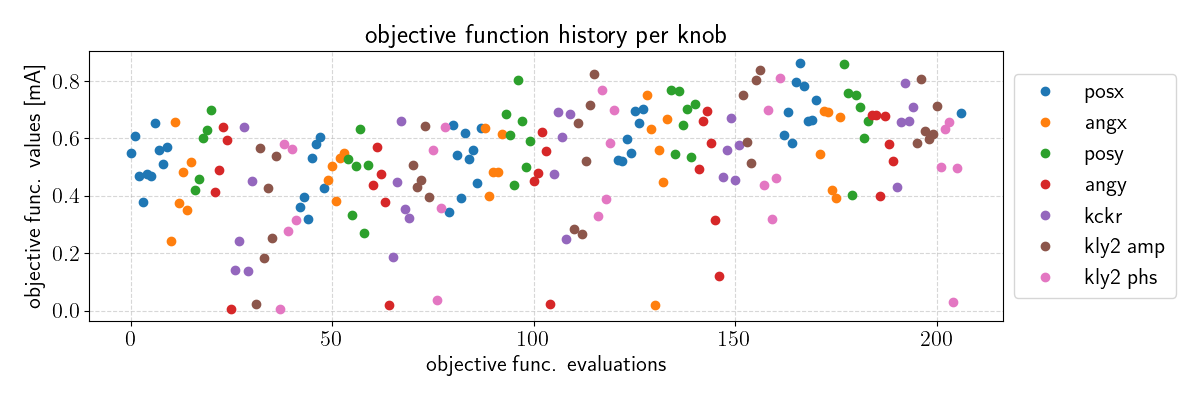
\includegraphics[width=\linewidth]{2024-07-12/figures/run1_history_by_knob.png}
    % \caption{Caption}
\end{figure}
\end{itemize}
\end{frame}
